%--------------------------------------
% Create title frame
\titleframe

%--------------------------------------
% Table of contents
\begin{frame}{Overview}
  \setbeamertemplate{section in toc}[sections numbered]
  \tableofcontents[hideallsubsections]
\end{frame}

%--------------------------------------
% What will we learn slide
\begin{frame}{What will we learn today?}
  \begin{itemize}
    \item What synchronous generators are and how they work.
    \item How we can model them for power system analyses.
    \item How to include generator capability limits in power flow computations.
  \end{itemize}
  \vspace{0.4cm}
  You will be able to solve exercises 9.5 to 9.9 of Ned Mohan's book:
  \begin{center}
    Mohan, Ned. \textit{Electric power systems: a first course}. John Wiley \& Sons, 2012.
  \end{center}
\end{frame}

%==============================================================================
% SECTION 1: Operating principle
%==============================================================================
\section{Operating principle}

\begin{frame}{Synchronous machines}
  Synchronous machines produce the major part of electrical energy worldwide:
  \begin{itemize}
    \item Unit ratings range from a few kVA (emergency generators) to a few hundred MVA, with the largest units exceeding 1500 MVA (nuclear power plants).
  \end{itemize}
  \vspace{0.2cm}
  Beyond bulk active power production, they play three critical system roles:
  \begin{itemize}
    \item \textbf{Frequency setting}: They impose the synchronous frequency of grid voltages and currents.
    \item \textbf{Energy buffer}: They store significant kinetic energy in their rotating masses (providing instantaneous system inertia).
    \item \textbf{Voltage control}: They can produce or consume reactive power by adjusting their rotor field current.
  \end{itemize}
\end{frame}

\begin{frame}{Magnetic field created by the stator}
  \begin{columns}
    \begin{column}{0.55\textwidth}
      \begin{itemize}
        \item \textbf{Stator (armature)}: Stationary outer structure separated from the rotor by a small air gap.
        \item Subjected to time-varying magnetic flux $\implies$ built from thin steel laminations to minimize \textbf{eddy (Foucault) currents}.
        \item Equipped with three windings ($a, b, c$) distributed $120^\circ$ apart in space.
        \item Magnetic field lines cross the air gap in a radial direction.
      \end{itemize}
    \end{column}
    \begin{column}{0.45\textwidth}
      \begin{center}
        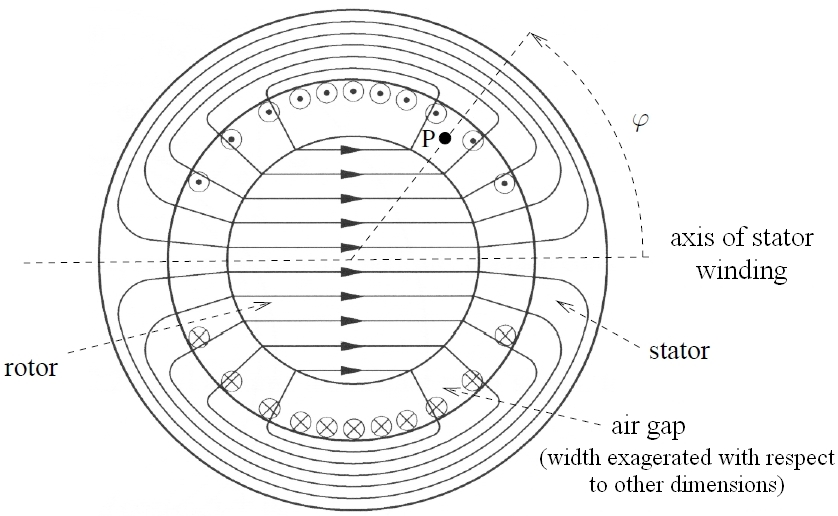
\includegraphics[height=0.45\textheight,keepaspectratio]{images/stator_field.jpg}\\
        \vspace{0.1cm}
        \tiny Field from direct current in one stator winding
      \end{center}
    \end{column}
  \end{columns}
\end{frame}

\begin{frame}{Three-phase stator winding layout}
  \begin{columns}
    \begin{column}{0.6\textwidth}
      The amplitude $B(\varphi)$ of the flux density along the air gap:
      \begin{itemize}
        \item Is a periodic function of spatial angle $\varphi$ with period $2\pi$.
        \item Has a discrete "staircase" shape in practice due to discrete slots.
        \item Is shaped as close as possible to a pure sinusoid by carefully distributing conductor coils along stator slots.
      \end{itemize}
    \end{column}
    \begin{column}{0.4\textwidth}
      \begin{center}
        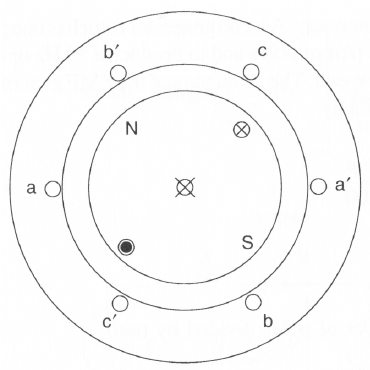
\includegraphics[height=0.5\textheight,keepaspectratio]{images/layout_phases.jpg}\\
        \vspace{0.1cm}
        \tiny Three-phase winding layout (single turn shown)
      \end{center}
    \end{column}
  \end{columns}
\end{frame}

\begin{frame}[allowframebreaks]{Rotating magnetic field}
  Total magnetic flux density created by the three phases at spatial angle $\varphi$:
  $$B_{3\phi}(\varphi) = k i_a \cos\varphi + k i_b \cos\left(\varphi - \frac{2\pi}{3}\right) + k i_c \cos\left(\varphi - \frac{4\pi}{3}\right)$$
  When balanced three-phase sinusoidal currents flow in the windings:
  \begin{align*}
    i_a(t) &= \sqrt{2} I \cos(\omega t + \psi) \\
    i_b(t) &= \sqrt{2} I \cos\left(\omega t + \psi - \frac{2\pi}{3}\right), \quad
    i_c(t) = \sqrt{2} I \cos\left(\omega t + \psi - \frac{4\pi}{3}\right)
  \end{align*}
  Using trigonometric identities:
  $$B_{3\phi}(\varphi, t) = \frac{3\sqrt{2} k I}{2} \cos(\omega t + \psi - \varphi)$$
  \begin{block}{Key conclusion}
    The three-phase AC currents together produce a magnetic field of constant amplitude rotating at electrical angular speed $\omega = 2\pi f$ (Ferraris theorem).
  \end{block}
\end{frame}

\begin{frame}{Magnetic field created by the rotor}
  \begin{columns}
    \begin{column}{0.55\textwidth}
      \begin{itemize}
        \item \textbf{Rotor}: The rotating cylindrical or salient part mounted on the turbine shaft.
        \item In steady state, a direct current ($I_f$) flows through the rotor winding.
        \item This winding is known as the \textbf{field winding} (\textit{enroulement d'excitation}).
        \item The DC current creates a magnetic field with alternating North and South poles that rotates along with the rotor.
      \end{itemize}
    \end{column}
    \begin{column}{0.45\textwidth}
      \begin{center}
        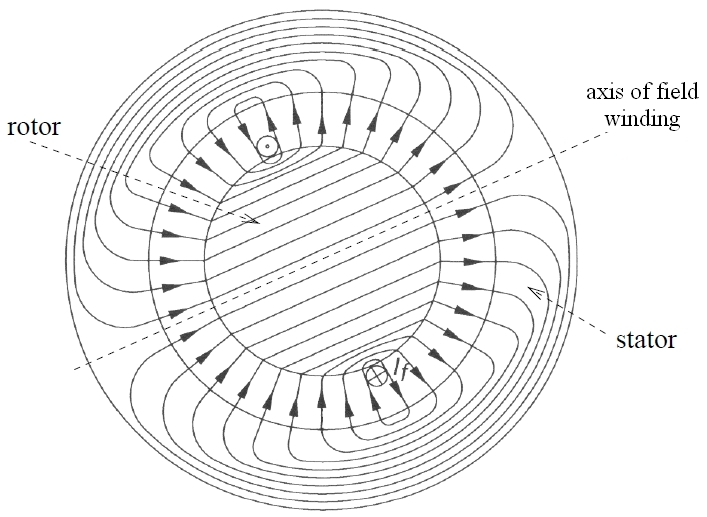
\includegraphics[height=0.55\textheight,keepaspectratio]{images/rotor_field.jpg}\\
        \vspace{0.1cm}
        \tiny Magnetic field produced by rotor field winding
      \end{center}
    \end{column}
  \end{columns}
\end{frame}

\begin{frame}{Interaction between fields \& electromechanical conversion}
  \begin{columns}
    \begin{column}{0.55\textwidth}
      \begin{itemize}
        \item In steady state, the rotor rotates at the exact same angular speed $\omega$ as the stator magnetic field: \textbf{synchronism}.
        \item Therefore, the stator and rotor magnetic fields are stationary with respect to each other.
        \item Both fields tend to align in the manner of two coupled magnets.
        \item Displacing them creates an electromagnetic torque $T_e$.
        \item There exists a maximum torque $T_{e,\max}$ beyond which synchronism is lost.
      \end{itemize}
    \end{column}
    \begin{column}{0.45\textwidth}
      \begin{center}
        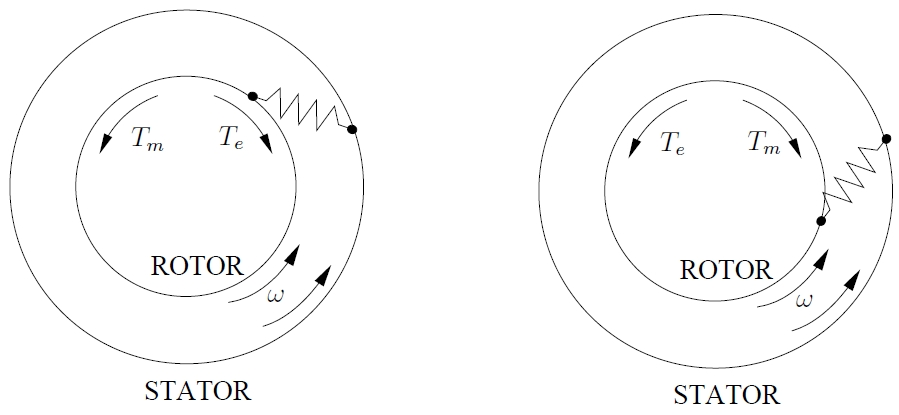
\includegraphics[height=0.45\textheight,keepaspectratio]{images/interaction_fields.jpg}\\
        \vspace{0.1cm}
        \small Mechanical analogy: generator mode $\leftrightarrow$ motor mode
      \end{center}
    \end{column}
  \end{columns}
\end{frame}

%==============================================================================
% SECTION 2: Types of synchronous machines
%==============================================================================
\section{Types of synchronous machines}

\begin{frame}{Machines with multiple pole pairs}
  \begin{columns}
    \begin{column}{0.55\textwidth}
      Certain prime movers (e.g. hydro turbines) run at low rotational speed, yet the electrical frequency must remain $f = 50\text{ Hz}$ ($T = 20\text{ ms}$):
      \begin{itemize}
        \item The rotor is equipped with $p$ pairs of poles ($2p$ poles).
        \item In one mechanical revolution, each stator winding experiences $p$ electrical cycles.
        \item Rotational speed $n$ (in rpm) is linked to grid frequency $f$:
          $$n = \frac{60 f}{p} = \frac{3000}{p}\text{ rpm} \quad (\text{at } 50\text{ Hz})$$
      \end{itemize}
    \end{column}
    \begin{column}{0.45\textwidth}
      \begin{center}
        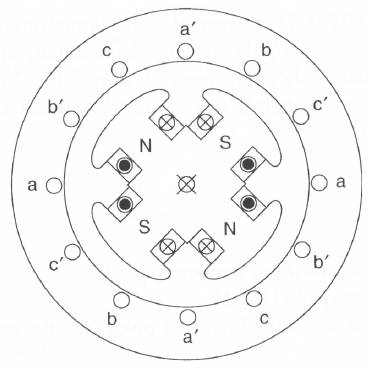
\includegraphics[height=0.55\textheight,keepaspectratio]{images/several_poles.jpg}\\
        \vspace{0.1cm}
        \small Example: $p = 2$ ($4$ poles, $n = 1500\text{ rpm}$)
      \end{center}
    \end{column}
  \end{columns}
\end{frame}

\begin{frame}{Round-rotor generators (turbo-alternators)}
  \begin{columns}
    \begin{column}{0.55\textwidth}
      Driven by high-speed steam or gas turbines:
      \begin{itemize}
        \item Typically $p=1$ ($3000\text{ rpm}$) or $p=2$ ($1500\text{ rpm}$ in nuclear plants).
        \item Cylindrical rotor forged from solid steel alloy; small diameter and long length (due to severe centrifugal forces).
        \item Field winding embedded in milled rotor slots.
        \item Extreme power density: cooled by pressurized hydrogen ($7\times$ higher thermal conductivity than air) or demineralized water in hollow conductors.
      \end{itemize}
    \end{column}
    \begin{column}{0.45\textwidth}
      \begin{center}
        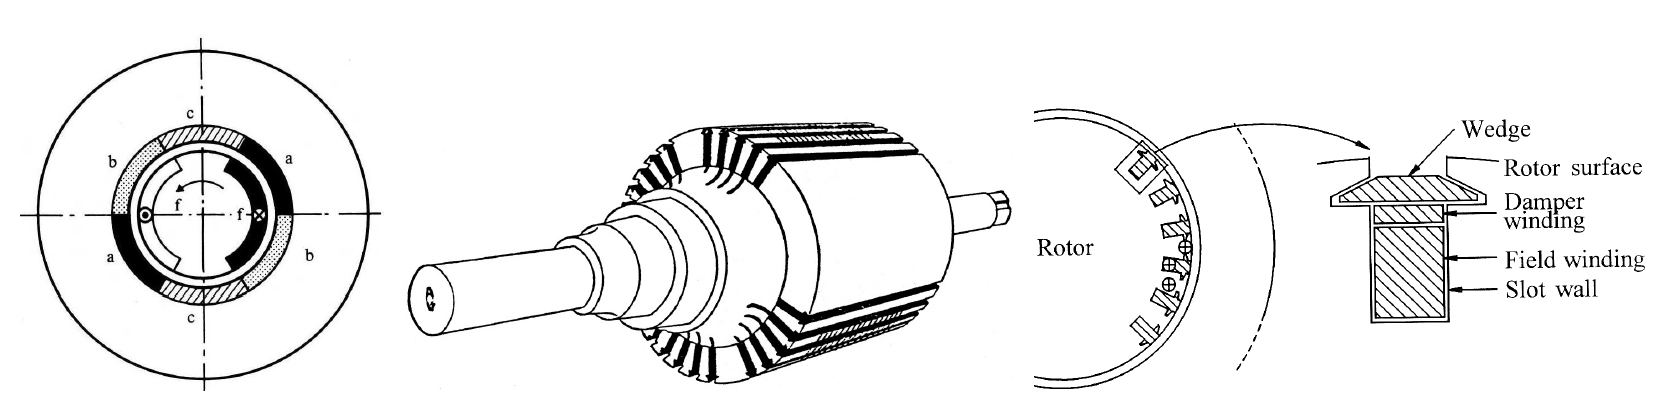
\includegraphics[height=0.55\textheight,keepaspectratio]{images/round_rotor.png}\\
        \vspace{0.1cm}
        \tiny Cross-section of a round-rotor machine
      \end{center}
    \end{column}
  \end{columns}
\end{frame}

\begin{frame}{Salient-pole generators}
  \begin{columns}
    \begin{column}{0.55\textwidth}
      Driven by low-speed hydraulic turbines or diesel engines:
      \begin{itemize}
        \item Number of pole pairs is large ($p \ge 4$, often $p \in [10, 40]$).
        \item Protruding (\textit{salient}) poles with concentrated field coils mounted on a large rotor wheel.
        \item Large diameter, short axial length.
        \item Rotor poles are made of laminated steel sheets.
        \item Usually cooled by natural or forced airflow around the rotor.
      \end{itemize}
    \end{column}
    \begin{column}{0.45\textwidth}
      \begin{center}
        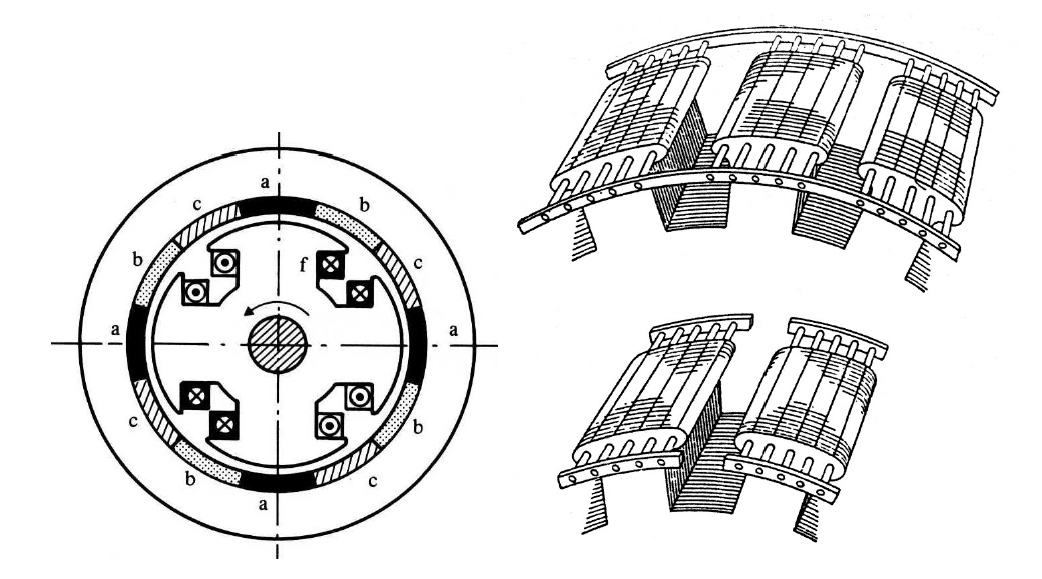
\includegraphics[height=0.55\textheight,keepaspectratio]{images/salient_poles.png}\\
        \vspace{0.1cm}
        \tiny Cross-section of a salient-pole machine
      \end{center}
    \end{column}
  \end{columns}
\end{frame}

\begin{frame}{Damper windings (\textit{amortisseurs})}
  \begin{itemize}
    \item Conductive bars (copper/brass) placed in rotor pole shoes and short-circuited at ends with rings (similar to a squirrel cage).
    \item \textbf{In steady state}:
      The stator and rotor magnetic fields rotate synchronously $\implies$ no relative motion, zero induced current in the dampers.
    \item \textbf{During a disturbance}:
      The rotor accelerates or decelerates relative to the synchronous magnetic field $\implies$ currents are induced in the damper bars.
    \item According to Lenz's law, these induced currents produce a \textbf{damping torque} that counteracts rotor oscillations and helps restore synchronism.
    \item In solid round-rotor machines, eddy currents flowing directly in the rotor steel provide a similar intrinsic damping effect.
  \end{itemize}
\end{frame}

%==============================================================================
% SECTION 3: Equivalent circuit and modeling
%==============================================================================
\section{Equivalent circuit and modeling}

\begin{frame}{Induced electromotive force (emf)}
  Two separate magnetic sources induce voltages in the stator windings:
  \begin{enumerate}
    \item \textbf{Excitation field}: The rotating rotor field induces an internal electromotive force (emf) denoted $\bar{E}_{af}$ (or open-circuit voltage).
    \item \textbf{Armature reaction}: The AC currents flowing in the stator windings produce their own magnetic field, inducing a voltage drop modeled as $-j X_s \bar{I}_a$.
  \end{enumerate}
  \vspace{0.3cm}
  Assuming no magnetic saturation, the resulting terminal phase voltage $\bar{V}_a$ is obtained by superposition:
  $$\bar{V}_a = \bar{E}_{af} - R_s \bar{I}_a - j X_s \bar{I}_a$$
  where $R_s$ is the stator winding resistance and $X_s$ is the \textbf{synchronous reactance}.
\end{frame}

\begin{frame}{Per-phase equivalent circuit}
  \begin{columns}
    \begin{column}{0.55\textwidth}
      \begin{center}
        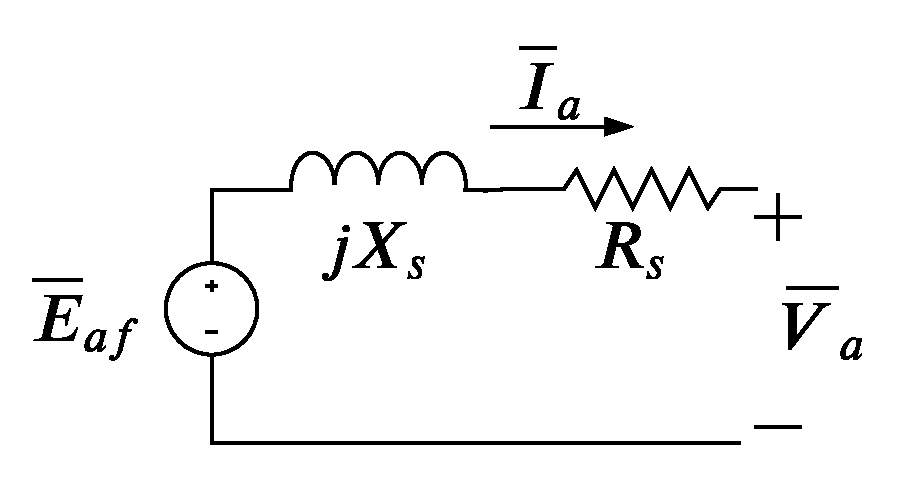
\includegraphics[width=0.95\textwidth]{images/generator_model.pdf}
      \end{center}
    \end{column}
    \begin{column}{0.45\textwidth}
      $$\bar{V}_a = \bar{E}_{af} - (R_s + j X_s)\bar{I}_a$$
      \begin{itemize}
        \item $R_s$: Stator resistance.
        \item $X_s$: Synchronous reactance (leakage + magnetizing reactance).
        \item $\delta$: Angle between $\bar{E}_{af}$ and $\bar{V}_a$, called the \textbf{internal angle} or \textbf{load angle}.
      \end{itemize}
    \end{column}
  \end{columns}
\end{frame}

\begin{frame}{Phasor diagram}
  \begin{columns}
    \begin{column}{0.55\textwidth}
      \begin{center}
        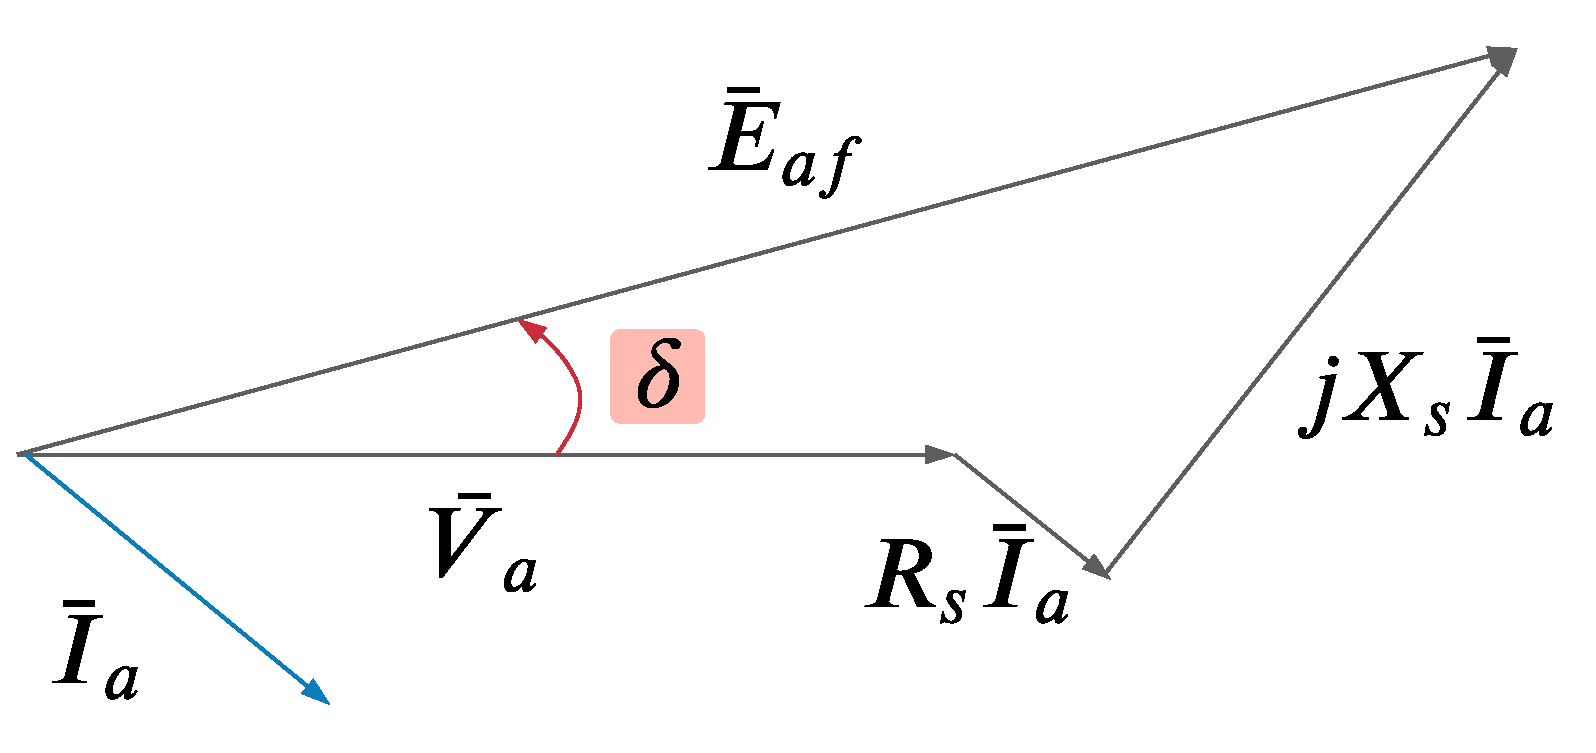
\includegraphics[width=\textwidth]{images/generator_diagram.pdf}
      \end{center}
    \end{column}
    \begin{column}{0.45\textwidth}
      \begin{itemize}
        \item $\bar{V}_a = V_a \angle 0^\circ$ is chosen as the reference.
        \item $\bar{I}_a$ is the stator phase current with phase lag $\phi$.
        \item Resistive drop $R_s \bar{I}_a$ is parallel to $\bar{I}_a$.
        \item Reactive drop $j X_s \bar{I}_a$ leads $\bar{I}_a$ by $90^\circ$.
        \item Vector sum yields the internal emf:
          $$\bar{E}_{af} = \bar{V}_a + R_s \bar{I}_a + j X_s \bar{I}_a$$
      \end{itemize}
    \end{column}
  \end{columns}
\end{frame}

\begin{frame}{Parameters and transient reactances}
  \textbf{Typical machine parameters (in per unit on machine rating base):}
  \begin{itemize}
    \item Stator resistance: $R_s \approx 0.005\text{ pu}$ (frequently neglected in grid studies).
    \item Synchronous reactance: $X_s \in [1.5, 2.5]\text{ pu}$ (for round-rotor turbo-generators).
  \end{itemize}
  \vspace{0.3cm}
  \textbf{Machine models for transient conditions:}
  Depending on the time frame of the phenomenon, stator reaction is hindered by rotor screening circuits:
  \begin{itemize}
    \item \textbf{Subtransient state} (first few cycles after a short circuit): $X''_s \ll X_s$ ($0.15 - 0.25\text{ pu}$).
    \item \textbf{Transient state} (hundreds of milliseconds): $X'_s < X_s$ ($0.25 - 0.40\text{ pu}$).
    \item \textbf{Steady state}: $X_s$ ($1.5 - 2.5\text{ pu}$).
  \end{itemize}
  $$\implies X''_s < X'_s < X_s$$
\end{frame}

%==============================================================================
% SECTION 4: Properties and reactive power control
%==============================================================================
\section{Properties and reactive power control}

\begin{frame}[allowframebreaks]{Power transfer to an external grid}
  Consider a generator connected to an infinite bus ($\bar{V}_\infty = V_\infty \angle 0^\circ$) through a step-up transformer and transmission line:
  \begin{center}
    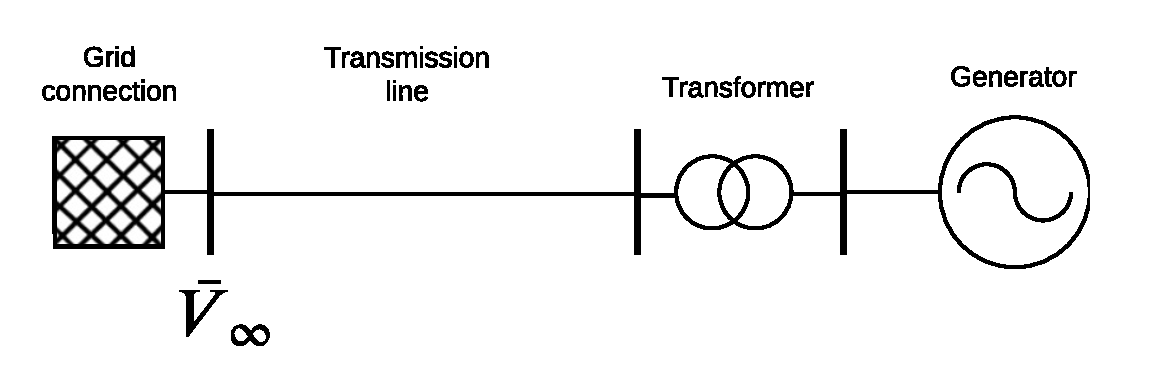
\includegraphics[width=0.75\textwidth]{images/generator_to_grid.pdf}
  \end{center}
  Neglecting resistances, let $X_T = X_s + X_{tr} + X_{line}$ be the total reactance between $\bar{E}_{af}$ and $\bar{V}_\infty$. The three-phase active power delivered to the grid is:
  $$P = \frac{E_{af} V_\infty}{X_T} \sin\delta$$
  where $\delta$ is the angle between internal emf $\bar{E}_{af}$ and infinite bus voltage $\bar{V}_\infty$.
\end{frame}

\begin{frame}{Steady-state stability limit}
  \begin{columns}
    \begin{column}{0.4\textwidth}
      \begin{center}
        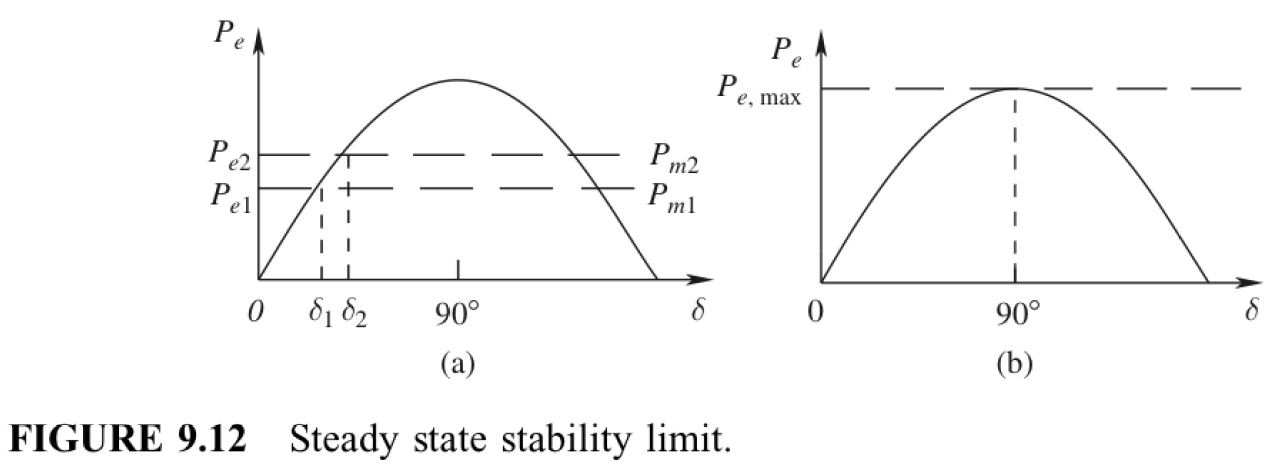
\includegraphics[width=\textwidth]{images/steady_state_stability_limit.png}
      \end{center}
    \end{column}
    \begin{column}{0.6\textwidth}
      \begin{itemize}
        \item When excitation $E_{af}$ is constant, active power $P$ is strictly proportional to $\sin\delta$.
        \item Maximum power is reached at $\delta = 90^\circ$:
          $$P_{\max} = \frac{E_{af} V_\infty}{X_T}$$
        \item For $\delta > 90^\circ$, $\frac{dP}{d\delta} < 0$: additional mechanical power causes rotor acceleration, increasing $\delta$ and reducing electrical power $\implies$ \alert{loss of synchronism}.
        \item In operation, $\delta$ is kept well below $90^\circ$, typically $\delta \le 40^\circ$.
      \end{itemize}
    \end{column}
  \end{columns}
\end{frame}

\begin{frame}{Adjusting reactive power via field current}
  Suppose the generator delivers constant active power $P$, requiring $E_{af} \sin\delta = \text{cst}$ and $I_a \cos\phi = \text{cst}$:
  \begin{center}
    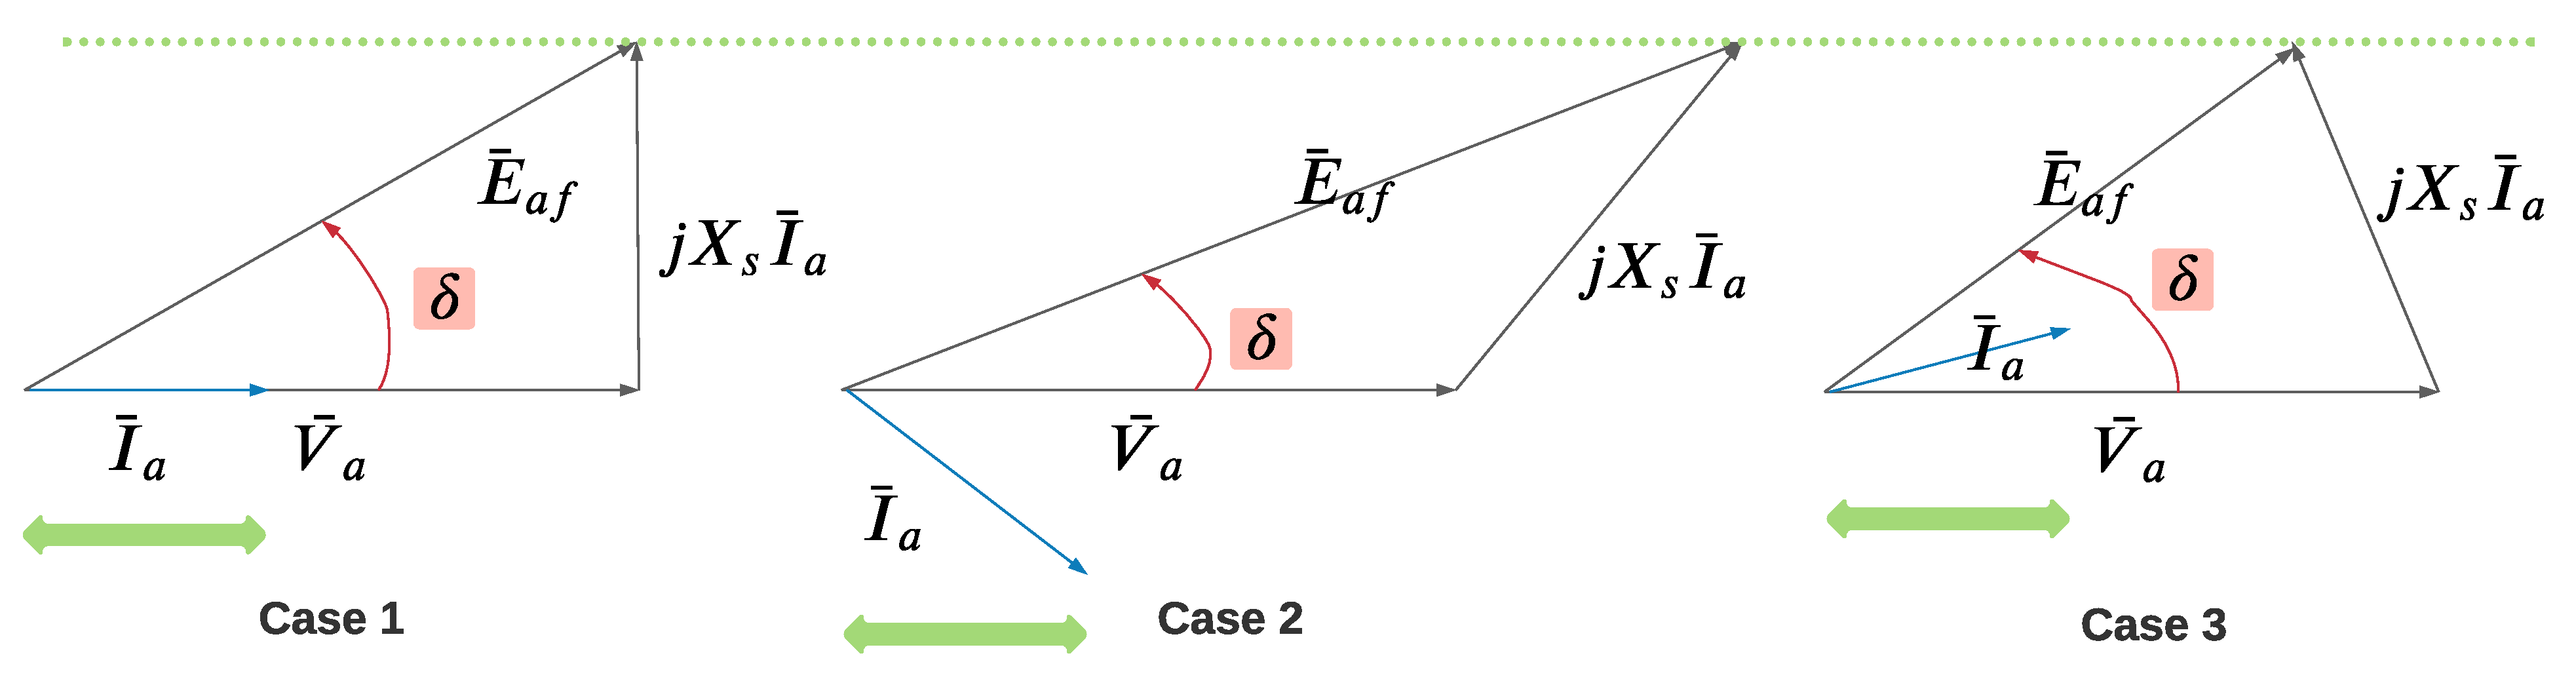
\includegraphics[width=0.85\textwidth]{images/adjusting_Q_diagram.pdf}
  \end{center}
  By varying the DC field excitation current $I_f$, we directly control the amplitude $E_{af}$ and the reactive power $Q$ exchanged with the grid.
\end{frame}

\begin{frame}{Overexcitation vs. Underexcitation}
  \begin{columns}
    \begin{column}{0.48\textwidth}
      \textbf{Overexcitation ($I_f \nearrow$, $E_{af} \nearrow$):}
      \begin{itemize}
        \item Current $\bar{I}_a$ lags terminal voltage $\bar{V}_a$ ($\phi > 0$).
        \item Generator \textbf{supplies} reactive power to the grid:
          $$Q = 3 V_a I_a \sin\phi > 0$$
        \item The generator behaves as a \textbf{capacitor} connected to the power system.
      \end{itemize}
    \end{column}
    \begin{column}{0.48\textwidth}
      \textbf{Underexcitation ($I_f \searrow$, $E_{af} \searrow$):}
      \begin{itemize}
        \item Current $\bar{I}_a$ leads terminal voltage $\bar{V}_a$ ($\phi < 0$).
        \item Generator \textbf{absorbs} reactive power from the grid:
          $$Q = 3 V_a I_a \sin\phi < 0$$
        \item The generator behaves as an \textbf{inductor} connected to the power system.
      \end{itemize}
    \end{column}
  \end{columns}
\end{frame}

\begin{frame}{Voltage regulation and synchronous condensers}
  \begin{itemize}
    \item \textbf{Automatic Voltage Regulation (AVR)}:
      \begin{itemize}
        \item Controls the DC rotor excitation current $I_f$ via feedback control.
        \item Dynamically adjusts internal emf $E_{af}$ and reactive power $Q$ to regulate the terminal bus voltage to a target setpoint $V_0$.
      \end{itemize}
    \vspace{0.3cm}
    \item \textbf{Synchronous Condensers}:
      \begin{itemize}
        \item Synchronous machines running without a mechanical load (drawing only enough active power to cover internal losses).
        \item Used exclusively to supply or absorb continuously variable reactive power and provide short-circuit power and inertia to the grid.
      \end{itemize}
  \end{itemize}
\end{frame}

\begin{frame}{Generator capability curve}
  The capability curve defines the permissible operating region in the $(P, Q)$ plane under constant terminal voltage $V$:
  \begin{center}
    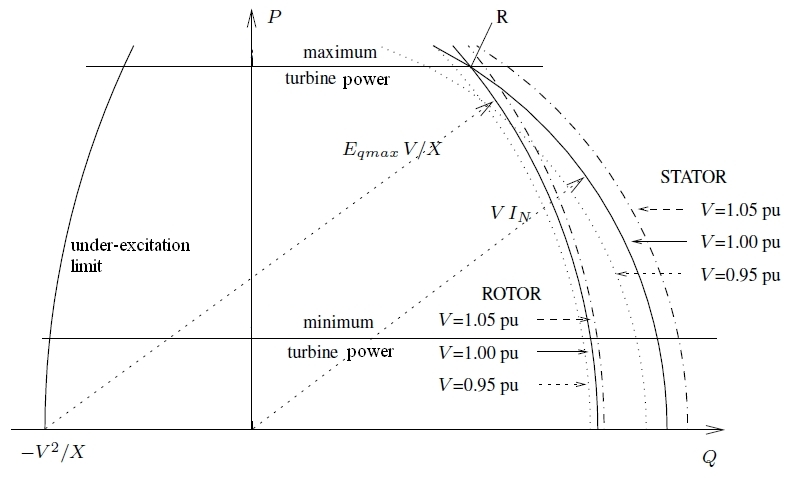
\includegraphics[height=0.62\textheight,keepaspectratio]{images/capability.jpg}
  \end{center}
\end{frame}

\begin{frame}{Operating limits breakdown}
  \begin{enumerate}
    \item \textbf{Prime mover (turbine) limit}: Maximum mechanical power input ($P \le P_{\max}$). A minimum power $P_{\min}$ also exists for flame stability in thermal boilers.
    \item \textbf{Stator thermal limit}: Armature Joule losses ($R_s I_a^2$). Current magnitude is capped ($I_a \le I_{a,\max}$):
      $$P^2 + Q^2 \le (V I_{a,\max})^2 \quad \text{(circle centered at origin)}$$
    \item \textbf{Rotor thermal limit}: Joule losses in field winding ($R_f I_f^2$). Maximum excitation voltage $E_{af} \le E_{af,\max}$:
      $$P^2 + \left(Q + \frac{V^2}{X_s}\right)^2 \le \left(\frac{V E_{af,\max}}{X_s}\right)^2 \quad \text{(circle centered at } (0, -V^2/X_s)\text{)}$$
    \item \textbf{Underexcitation / Stability limit}: Minimum field excitation required to avoid excessive internal angle $\delta$ and loss of synchronism.
  \end{enumerate}
\end{frame}

%==============================================================================
% SECTION 5: Power flow analysis
%==============================================================================
\section{Generators in power flow analysis}

\begin{frame}{Inclusion in power flow: PV to PQ bus switching}
  In power flow formulations:
  \begin{itemize}
    \item A synchronous generator is initially modeled as a \textbf{PV bus}:
      \begin{itemize}
        \item Active power $P$ is fixed by turbine dispatch.
        \item Voltage magnitude $|V|$ is fixed by the AVR setpoint.
        \item Reactive power $Q$ and phase angle $\theta$ are unknown.
      \end{itemize}
    \item After computing power flow equations, the required reactive power $Q$ is checked against capability limits:
      $$Q_{\min} \le Q \le Q_{\max}$$
    \item If a limit is violated (e.g. $Q > Q_{\max}$):
      \begin{itemize}
        \item The generator cannot provide enough field current to sustain the voltage setpoint.
        \item The bus is switched from a \textbf{PV bus} to a \textbf{PQ bus} with $Q = Q_{\max}$ (or $Q_{\min}$).
        \item Voltage $|V|$ is freed and becomes a state variable.
        \item Power flow is re-solved iteratively until no limits are violated.
      \end{itemize}
  \end{itemize}
\end{frame}

\begin{frame}{Simulation with PandaPower}
  In PandaPower, generator limits can be directly enforced during AC power flow calculations:
  \vspace{0.3cm}
  \begin{center}
    \texttt{pp.runpp(net, enforce\_q\_limits=True)}
  \end{center}
  \vspace{0.3cm}
  \begin{tcolorbox}[colback=blue!5,colframe=blue!75,title=Google Colab Notebook]
    \centering
    Explore synchronous machine modeling and PV/PQ switching in PandaPower:\\
    \url{https://colab.research.google.com/drive/1Q9E62wzrKiCsBIyRH9JnCTMSibSlY9OG?usp=sharing}
  \end{tcolorbox}
\end{frame}

\begin{frame}{References}
  \begin{itemize}
    \item Course notes of ELEC0014 (\textit{Electric Energy Systems}) by Pr. Thierry Van Cutsem, University of Liège.
    \item Mohan, Ned. \textit{Electric power systems: a first course}. John Wiley \& Sons, 2012.
    \item L. Thurner, A. Scheidler, F. Schäfer et al., "pandapower - an Open Source Python Tool for Convenient Modeling, Analysis and Optimization of Electric Power Systems", \textit{IEEE Transactions on Power Systems}, vol. 33, no. 6, pp. 6510-6521, Nov. 2018.
  \end{itemize}
\end{frame}
